---
id: tkz-euclide-ejemplo-61
title: "Circunferencia y sector circular"
description: "Creación de una circunferencia y sectores circulares"
keywords: [circunferencia, sector, circular,taller4]
tags: [tkzDrawCircle,tkzDefPointOnCircle,tkzFillSector]
sort: 61
---
\documentclass[tikz,border=2mm]{standalone}
\usepackage{tkz-base}
\usepackage{tkz-euclide}

\begin{document}
    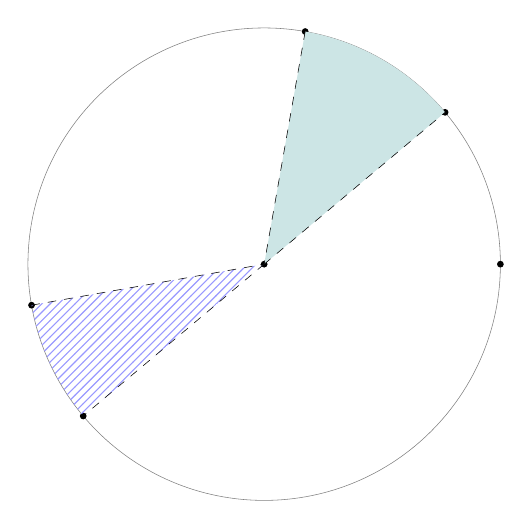
\begin{tikzpicture}        
        % Paso 1: Define puntos de un radio.
        \tkzDefPoint(5,5){O} % Punto central
        \tkzDefPoint(8,5){A} % Punto de circunferencia

        % Paso 2: Dibuja la circunferencia
        \tkzDrawCircle(O,A)        

        % Paso 3: Define punto B en la circunferencia
        % a 40 grados del punto A
        \tkzDefPointOnCircle[through=center O angle 40 point A]
             \tkzGetPoint{B}
             
        % Paso 4: Define punto C en la circunferencia
        % a 80 grados del punto A
        \tkzDefPointOnCircle[through=center O angle 80 point A]
            \tkzGetPoint{C}

        % Paso 5: Define punto D en la circunferencia
        % a 190 grados del punto A
        \tkzDefPointOnCircle[through=center O angle 190 point A]
            \tkzGetPoint{D}

        % Paso 6: Define punto E en la circunferencia
        % a 220 grados del punto A            
        \tkzDefPointOnCircle[through=center O angle 220 point A]
            \tkzGetPoint{E}

        % Paso 7: Dibuja los puntos A,B,C,D,E en la circunferencia
        \tkzDrawPoints(O,A,B,C,D,E)

        % Paso 8: Rellena sector OB->C de color turquesa, opacidad 20%
        \tkzFillSector[teal!20](O,B)(C)

        % Paso 9: Rellena sector OD->E de un patrón de lineas azules
        \tkzFillSector[pattern=north east lines, pattern color=blue!40](O,D)(E)

        % Paso 10: Dibuja rayos OC y OB para resaltar sector circular
        \tkzDrawSegments[dashed](C,O O,B)

        % Paso 11: Dibuja rayos OD y OE para resaltar sector circular
        \tkzDrawSegments[dashed](D,O O,E)        
    \end{tikzpicture}
\end{document}